\documentclass[]{article}
\usepackage{lmodern}
\usepackage{amssymb,amsmath}
\usepackage{ifxetex,ifluatex}
\usepackage{fixltx2e} % provides \textsubscript
\ifnum 0\ifxetex 1\fi\ifluatex 1\fi=0 % if pdftex
  \usepackage[T1]{fontenc}
  \usepackage[utf8]{inputenc}
\else % if luatex or xelatex
  \ifxetex
    \usepackage{mathspec}
    \usepackage{xltxtra,xunicode}
  \else
    \usepackage{fontspec}
  \fi
  \defaultfontfeatures{Mapping=tex-text,Scale=MatchLowercase}
  \newcommand{\euro}{€}
\fi
% use upquote if available, for straight quotes in verbatim environments
\IfFileExists{upquote.sty}{\usepackage{upquote}}{}
% use microtype if available
\IfFileExists{microtype.sty}{%
\usepackage{microtype}
\UseMicrotypeSet[protrusion]{basicmath} % disable protrusion for tt fonts
}{}
\usepackage[margin=1in]{geometry}
\usepackage{color}
\usepackage{fancyvrb}
\newcommand{\VerbBar}{|}
\newcommand{\VERB}{\Verb[commandchars=\\\{\}]}
\DefineVerbatimEnvironment{Highlighting}{Verbatim}{commandchars=\\\{\}}
% Add ',fontsize=\small' for more characters per line
\usepackage{framed}
\definecolor{shadecolor}{RGB}{248,248,248}
\newenvironment{Shaded}{\begin{snugshade}}{\end{snugshade}}
\newcommand{\KeywordTok}[1]{\textcolor[rgb]{0.13,0.29,0.53}{\textbf{{#1}}}}
\newcommand{\DataTypeTok}[1]{\textcolor[rgb]{0.13,0.29,0.53}{{#1}}}
\newcommand{\DecValTok}[1]{\textcolor[rgb]{0.00,0.00,0.81}{{#1}}}
\newcommand{\BaseNTok}[1]{\textcolor[rgb]{0.00,0.00,0.81}{{#1}}}
\newcommand{\FloatTok}[1]{\textcolor[rgb]{0.00,0.00,0.81}{{#1}}}
\newcommand{\CharTok}[1]{\textcolor[rgb]{0.31,0.60,0.02}{{#1}}}
\newcommand{\StringTok}[1]{\textcolor[rgb]{0.31,0.60,0.02}{{#1}}}
\newcommand{\CommentTok}[1]{\textcolor[rgb]{0.56,0.35,0.01}{\textit{{#1}}}}
\newcommand{\OtherTok}[1]{\textcolor[rgb]{0.56,0.35,0.01}{{#1}}}
\newcommand{\AlertTok}[1]{\textcolor[rgb]{0.94,0.16,0.16}{{#1}}}
\newcommand{\FunctionTok}[1]{\textcolor[rgb]{0.00,0.00,0.00}{{#1}}}
\newcommand{\RegionMarkerTok}[1]{{#1}}
\newcommand{\ErrorTok}[1]{\textbf{{#1}}}
\newcommand{\NormalTok}[1]{{#1}}
\usepackage{graphicx}
\makeatletter
\def\maxwidth{\ifdim\Gin@nat@width>\linewidth\linewidth\else\Gin@nat@width\fi}
\def\maxheight{\ifdim\Gin@nat@height>\textheight\textheight\else\Gin@nat@height\fi}
\makeatother
% Scale images if necessary, so that they will not overflow the page
% margins by default, and it is still possible to overwrite the defaults
% using explicit options in \includegraphics[width, height, ...]{}
\setkeys{Gin}{width=\maxwidth,height=\maxheight,keepaspectratio}
\ifxetex
  \usepackage[setpagesize=false, % page size defined by xetex
              unicode=false, % unicode breaks when used with xetex
              xetex]{hyperref}
\else
  \usepackage[unicode=true]{hyperref}
\fi
\hypersetup{breaklinks=true,
            bookmarks=true,
            pdfauthor={},
            pdftitle={U.S. Most Dangerous Storms},
            colorlinks=true,
            citecolor=blue,
            urlcolor=blue,
            linkcolor=magenta,
            pdfborder={0 0 0}}
\urlstyle{same}  % don't use monospace font for urls
\setlength{\parindent}{0pt}
\setlength{\parskip}{6pt plus 2pt minus 1pt}
\setlength{\emergencystretch}{3em}  % prevent overfull lines
\setcounter{secnumdepth}{0}

%%% Use protect on footnotes to avoid problems with footnotes in titles
\let\rmarkdownfootnote\footnote%
\def\footnote{\protect\rmarkdownfootnote}

%%% Change title format to be more compact
\usepackage{titling}

% Create subtitle command for use in maketitle
\newcommand{\subtitle}[1]{
  \posttitle{
    \begin{center}\large#1\end{center}
    }
}

\setlength{\droptitle}{-2em}
  \title{U.S. Most Dangerous Storms}
  \pretitle{\vspace{\droptitle}\centering\huge}
  \posttitle{\par}
  \author{}
  \preauthor{}\postauthor{}
  \date{}
  \predate{}\postdate{}



\begin{document}

\maketitle


\section{Synopsis}\label{synopsis}

Through the exploration of U.S. National Oceanic and Atmospheric
Administration's (NOAA) storm database, we have discovered Tornadoes are
the most harmful type of storm to the population's health, while the
Floods are the greatest economical consequences causing storm. The
criteria to be classified as the most harmful storm is: the highest
totals of fatalities and injuries caused throughout the times
(1950-2011). The criteria to be classified as the greatest economical
consequences causing storm is: the highest total property and crop
damages throughout the times (1950-2011).

\section{Data Processing}\label{data-processing}

For this analysis, we will be using the U.S. National Oceanic and
Atmospheric Administration's (NOAA) storm database. The tools we will
use are: RStudio and knitr.

Firstly, download the raw data and upload it.

\begin{Shaded}
\begin{Highlighting}[]
\NormalTok{myStormDataRaw <-}\StringTok{ }\KeywordTok{read.csv}\NormalTok{(}\KeywordTok{bzfile}\NormalTok{(}\StringTok{"repdata_data_StormData.csv.bz2"}\NormalTok{))}
\end{Highlighting}
\end{Shaded}

\subsubsection{Data Clean Up}\label{data-clean-up}

We notice our attribute EVTYPE which identifies the type of storm,is not
consistent with naming convention. We will we will perform few simple
data clean up techniques to give ourselves less unique storm types.

Make the desired fields to upper case to ensure aggregation and grouping
works as expected.

\begin{Shaded}
\begin{Highlighting}[]
\NormalTok{myStormDataRaw$EVTYPE <-}\StringTok{ }\KeywordTok{toupper}\NormalTok{(myStormDataRaw$EVTYPE)}
\NormalTok{myStormDataRaw$PROPDMGEXP <-}\StringTok{ }\KeywordTok{toupper}\NormalTok{(myStormDataRaw$PROPDMGEXP)}
\NormalTok{myStormDataRaw$CROPDMGEXP <-}\StringTok{ }\KeywordTok{toupper}\NormalTok{(myStormDataRaw$CROPDMGEXP)}
\end{Highlighting}
\end{Shaded}

Remove punctuations (ex: ``('', ``/'', etc.) to increase the accuracy of
grouping.

\begin{Shaded}
\begin{Highlighting}[]
\NormalTok{myStormDataRaw$EVTYPE <-}\StringTok{ }\KeywordTok{gsub}\NormalTok{(}\StringTok{"[[:punct:]+]"}\NormalTok{, }\StringTok{""}\NormalTok{, myStormDataRaw$EVTYPE)}
\end{Highlighting}
\end{Shaded}

We will also convert PROPDMGEXP and CROPDMGEXP into their respective
values. IE. B = 1,000,000,000; M = 1,000,000; K = 1,000; H = 100. This
will allow us to combine this field with PROPDMG and CROPDMG to get the
true values for damages.

\begin{Shaded}
\begin{Highlighting}[]
\NormalTok{myStormDataRaw$PROPDMGEXP <-}\StringTok{ }\KeywordTok{gsub}\NormalTok{(}\StringTok{"B"}\NormalTok{, }\DecValTok{1000000000}\NormalTok{, myStormDataRaw$PROPDMGEXP)}
\NormalTok{myStormDataRaw$PROPDMGEXP <-}\StringTok{ }\KeywordTok{gsub}\NormalTok{(}\StringTok{"M"}\NormalTok{, }\DecValTok{1000000}\NormalTok{, myStormDataRaw$PROPDMGEXP)}
\NormalTok{myStormDataRaw$PROPDMGEXP <-}\StringTok{ }\KeywordTok{gsub}\NormalTok{(}\StringTok{"K"}\NormalTok{, }\DecValTok{1000}\NormalTok{, myStormDataRaw$PROPDMGEXP)}
\NormalTok{myStormDataRaw$PROPDMGEXP <-}\StringTok{ }\KeywordTok{gsub}\NormalTok{(}\StringTok{"H"}\NormalTok{, }\DecValTok{100}\NormalTok{, myStormDataRaw$PROPDMGEXP)}
\NormalTok{myStormDataRaw$PROPDMGEXP <-}\StringTok{ }\KeywordTok{as.numeric}\NormalTok{(myStormDataRaw$PROPDMGEXP)}
\end{Highlighting}
\end{Shaded}

\begin{verbatim}
## Warning: NAs introduced by coercion
\end{verbatim}

Perform the changes as above for CROPDMGEXP.

\begin{Shaded}
\begin{Highlighting}[]
\NormalTok{myStormDataRaw$CROPDMGEXP <-}\StringTok{ }\KeywordTok{gsub}\NormalTok{(}\StringTok{"B"}\NormalTok{, }\DecValTok{1000000000}\NormalTok{, myStormDataRaw$CROPDMGEXP)}
\NormalTok{myStormDataRaw$CROPDMGEXP <-}\StringTok{ }\KeywordTok{gsub}\NormalTok{(}\StringTok{"M"}\NormalTok{, }\DecValTok{1000000}\NormalTok{, myStormDataRaw$CROPDMGEXP)}
\NormalTok{myStormDataRaw$CROPDMGEXP <-}\StringTok{ }\KeywordTok{gsub}\NormalTok{(}\StringTok{"K"}\NormalTok{, }\DecValTok{1000}\NormalTok{, myStormDataRaw$CROPDMGEXP)}
\NormalTok{myStormDataRaw$CROPDMGEXP <-}\StringTok{ }\KeywordTok{gsub}\NormalTok{(}\StringTok{"H"}\NormalTok{, }\DecValTok{100}\NormalTok{, myStormDataRaw$CROPDMGEXP)}
\NormalTok{myStormDataRaw$CROPDMGEXP <-}\StringTok{ }\KeywordTok{as.numeric}\NormalTok{(myStormDataRaw$CROPDMGEXP)}
\end{Highlighting}
\end{Shaded}

\begin{verbatim}
## Warning: NAs introduced by coercion
\end{verbatim}

\subsection{1. The most harmful storm with respect to population
health}\label{the-most-harmful-storm-with-respect-to-population-health}

In this analysis, the criteria to be classified as the most harmful
storm is: the highest totals of fatalities and injuries caused
throughout the times.

Set myHarmfulStorm to be the total sum of fatalities and injuries caused
by each type of storm.Sum the values, ignore NA values.

\begin{Shaded}
\begin{Highlighting}[]
\NormalTok{myHarmfulStorm <-}\StringTok{ }\KeywordTok{aggregate}\NormalTok{(}\KeywordTok{list}\NormalTok{(}\DataTypeTok{TotalHarm =} \NormalTok{myStormDataRaw$FATALITIES +}\StringTok{ }\NormalTok{myStormDataRaw$INJURIES), }\KeywordTok{list}\NormalTok{(}\DataTypeTok{Storm=}\NormalTok{myStormDataRaw$EVTYPE), }\DataTypeTok{FUN=}\NormalTok{sum, }\DataTypeTok{na.rm=}\OtherTok{TRUE}\NormalTok{)}
\end{Highlighting}
\end{Shaded}

Display top 5 in descending order (note: only care for the number one
spot).

\begin{Shaded}
\begin{Highlighting}[]
\KeywordTok{head}\NormalTok{(myHarmfulStorm[}\KeywordTok{order}\NormalTok{(-myHarmfulStorm$TotalHarm),],}\DecValTok{5}\NormalTok{)}
\end{Highlighting}
\end{Shaded}

\begin{verbatim}
##              Storm TotalHarm
## 739        TORNADO     96979
## 116 EXCESSIVE HEAT      8428
## 760      TSTM WIND      7461
## 153          FLOOD      7259
## 407      LIGHTNING      6047
\end{verbatim}

For visual comparison to understand how much greater Tornado is compared
to the next 4 most dangers storms.

\begin{Shaded}
\begin{Highlighting}[]
\KeywordTok{barplot}\NormalTok{(}\KeywordTok{head}\NormalTok{(myHarmfulStorm[}\KeywordTok{order}\NormalTok{(-myHarmfulStorm$TotalHarm),],}\DecValTok{5}\NormalTok{)$TotalHarm, }\DataTypeTok{main=}\StringTok{"Total Harm"}\NormalTok{, }\DataTypeTok{xlab=}\StringTok{"Rank order (left to right)"}\NormalTok{, }\DataTypeTok{ylab=}\StringTok{"Total Harm"}\NormalTok{)}
\end{Highlighting}
\end{Shaded}

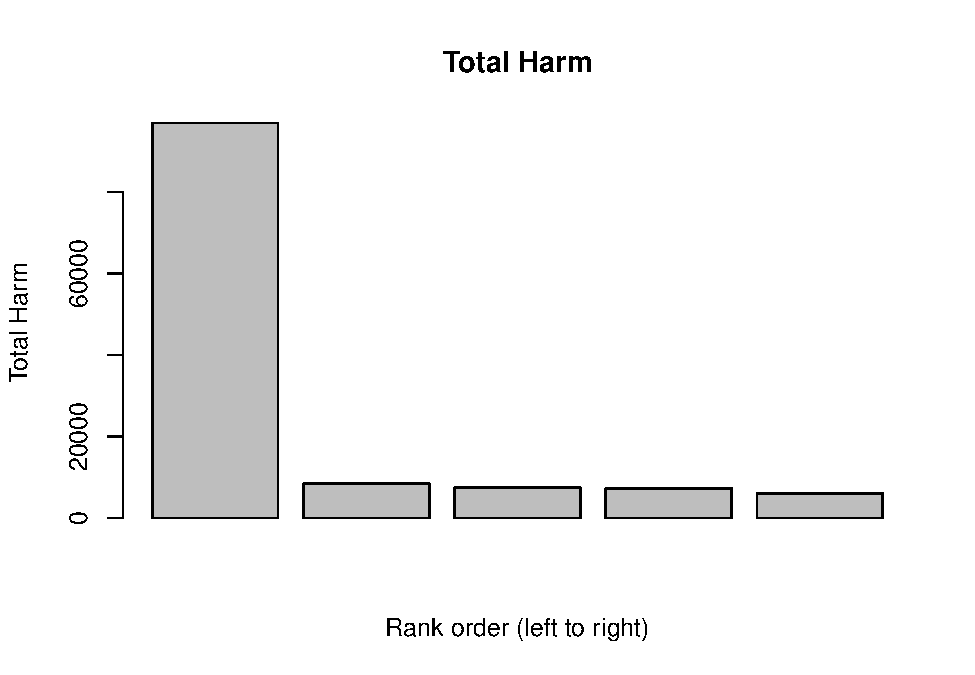
\includegraphics{pa2_files/figure-latex/unnamed-chunk-8-1.pdf}

\subsection{2. The greatest economical consequences causing
storm}\label{the-greatest-economical-consequences-causing-storm}

In this analysis, the criteria to be classified as the greatest
economical consequences causing storm is: the highest total property and
crop damages throughout the times.

Set myEcoCons to be the total sum of property and crop damages done by
each type of storm. Multiple the PROPDMG with PROPDMGEXP to get real
value, and multiple CROPDMG and CROPDMGEXP, sum values, ignore NA
values.

\begin{Shaded}
\begin{Highlighting}[]
\NormalTok{myEcoCons <-}\StringTok{ }\KeywordTok{aggregate}\NormalTok{(}\KeywordTok{list}\NormalTok{(}\DataTypeTok{TotalDamage =} \KeywordTok{as.numeric}\NormalTok{(myStormDataRaw$PROPDMG*myStormDataRaw$PROPDMGEXP) +}\StringTok{ }\KeywordTok{as.numeric}\NormalTok{(myStormDataRaw$CROPDMG*myStormDataRaw$CROPDMGEXP)), }\KeywordTok{list}\NormalTok{(}\DataTypeTok{Storm =} \NormalTok{myStormDataRaw$EVTYPE), }\DataTypeTok{FUN=}\NormalTok{sum, }\DataTypeTok{na.rm=}\OtherTok{TRUE}\NormalTok{)}
\end{Highlighting}
\end{Shaded}

Display top 5 in descending order (note: only care for the number one
spot).

\begin{Shaded}
\begin{Highlighting}[]
\KeywordTok{head}\NormalTok{(myEcoCons[}\KeywordTok{order}\NormalTok{(-myEcoCons$TotalDamage),],}\DecValTok{5}\NormalTok{)}
\end{Highlighting}
\end{Shaded}

\begin{verbatim}
##                Storm  TotalDamage
## 153            FLOOD 138007444500
## 361 HURRICANETYPHOON  29348167800
## 739          TORNADO  16570326150
## 352        HURRICANE  12405268000
## 517      RIVER FLOOD  10108369000
\end{verbatim}

\section{Results}\label{results}

Shown by the numbers of fatalities and injuries caused, Tornado is the
most harmful storm that caused 96,979 fatalities and injuries. Through
the numbers of property and crop damages, Flood is the most economical
consequences causing storm that caused \$138,007,444,500 property damage
and crop damage.

\end{document}
